\documentclass[11pt]{article}

\usepackage[utf8]{inputenc}
\usepackage[T1]{fontenc}
\usepackage{booktabs}
\usepackage{graphicx}
\usepackage{amsmath, amssymb}
\usepackage{hyperref}
\usepackage[margin=1in]{geometry}
\usepackage{xcolor}

% TODO(author): swap in your target venue's class file (e.g. neurips_2024, acl, etc.) --
% this is a generic article skeleton so it compiles standalone with pdflatex.

\newcommand{\todo}[1]{\textcolor{red}{\textbf{TODO: #1}}}

\title{Communication-Efficient Federated Fine-Tuning of Medical Foundation Models\\
under Cross-Specialty Heterogeneity}
\author{\todo{author names / affiliations}}
\date{}

\begin{document}
\maketitle

\begin{abstract}
Federated fine-tuning lets multiple hospitals collaboratively adapt a shared medical imaging
backbone without pooling patient data, but cross-specialty heterogeneity -- where each hospital's
data distribution reflects a different medical specialty rather than a random partition of one
distribution -- breaks the implicit i.i.d.\ assumption behind naive aggregation schemes like
FedAvg. We study this setting with a fully simulated, CPU-only pipeline: five MedMNIST specialty
subsets (pathology, dermatology, blood, retina, kidney tissue) stand in for five hospitals, and
each client fine-tunes a frozen pretrained image backbone via LoRA adapters, communicating only
the low-rank adapter factors. We propose \textbf{FedSAA} (Similarity-Attended Aggregation), which
forms each client's merged LoRA delta $U_i = B_iA_i$, computes a softmax-attention aggregate over
other clients' deltas weighted by cosine similarity, blends it with the uniform mean via a
$\lambda$ parameter, and re-factorizes the result to a personalized rank-$r$ adapter per client
via truncated SVD. FedSAA reduces exactly to FedAvg-on-merged-deltas at $\lambda=1$ (proved in
\texttt{tests/test\_fedsaa.py}). On our \texttt{local\_debug} smoke configuration, FedSAA improves
global accuracy, macro-F1, AUC, and worst-client accuracy over FedAvg and FedProx at identical
communication cost. \todo{replace/extend once full\_run.yaml results are in -- current numbers
are from the reduced debug pipeline, not the intended full-scale experiment.}
\end{abstract}

\section{Introduction}
\todo{motivate the clinical/practical framing in your own words -- why cross-specialty (vs.
cross-institution-same-specialty) heterogeneity is under-studied, why LoRA-based
parameter-efficient FL matters for hospital-side compute/communication budgets, and what gap
FedSAA fills relative to FedAvg/FedProx.}

Contributions (as implemented in this codebase):
\begin{enumerate}
  \item A CPU-only, fully reproducible simulation harness (\texttt{src/data}, \texttt{src/models},
    \texttt{src/federated}) mapping five MedMNIST specialty subsets to five simulated hospitals
    under a shared config schema (\texttt{configs/local\_debug.yaml}, \texttt{configs/full\_run.yaml}).
  \item \textbf{FedSAA} (\texttt{src/federated/fedsaa.py}), a similarity-attended LoRA aggregation
    rule that personalizes each client's adapter via softmax attention over cosine similarity of
    merged LoRA deltas, with a provable reduction to FedAvg at $\lambda=1$.
  \item An evaluation suite (\texttt{src/metrics}) covering accuracy/macro-F1/AUC, communication
    accounting, and linear-CKA representation-collapse tracking, plus an ablation and
    table/figure generation pipeline (\texttt{experiments/}, \texttt{src/viz/}).
\end{enumerate}
\todo{add 1-2 more paragraphs of narrative framing / related-work teaser.}

\section{Related Work}
\todo{placeholder citation keys below -- fill in real citations and comparison sentences.}

\subsection{Federated Learning}
FedAvg~\cite{mcmahan2017fedavg} established sample-weighted parameter averaging as the default
aggregation rule; FedProx~\cite{li2020fedprox} adds a proximal term to stabilize local updates
under statistical heterogeneity. Both are implemented here as baselines
(\texttt{src/federated/loop.py}, \texttt{client.py}) for direct, same-codebase comparison.

\subsection{LoRA / Parameter-Efficient Fine-Tuning (PEFT)}
LoRA~\cite{hu2021lora} freezes a pretrained backbone and injects trainable low-rank factors
$(A,B)$ into target layers -- in our setup, 148{,}309 trainable parameters (1.31\% of the
11.3M-parameter ResNet-18 + head) per client, and a 0.548\,MB adapter payload (Table~\ref{tab:efficiency}).
Naively averaging LoRA factors $(A_i,B_i)$ directly is a biased approximation of averaging the
effective weight update; FedSAA's $\lambda=1$ case is explicitly defined at the level of merged
deltas $U_i=B_iA_i$ to sidestep this (Section~\ref{sec:method-fedavg-equiv}).

\subsection{Federated Learning in Medical Imaging}
\todo{cite medical FL surveys / cross-silo hospital FL work; discuss how those typically assume a
shared task/label space, unlike our cross-specialty setting where each client has a different
specialty and different \#classes (Table~\ref{tab:hyperparameters}).}

\subsection{Personalized Federated Learning}
FedSAA produces a genuinely personalized adapter per client (unlike FedAvg/FedProx's single
global adapter) via attention over client similarity. \todo{cite personalized/clustered-FL
baselines and position FedSAA's per-layer, per-round attention mechanism relative to them.}

\section{Method: FedSAA (Similarity-Attended Aggregation)}
\label{sec:method}

Let client $i \in \{1,\dots,n\}$ hold LoRA factors $(A_i, B_i)$ for a given target layer after
local training. Per round, per layer, the server
(\texttt{src/federated/fedsaa.py::fedsaa\_aggregate}) computes:

\begin{align}
  U_i &= B_i A_i \quad \text{(flattened)} \label{eq:merge} \\
  S_{ij} &= \cos(U_i, U_j) \label{eq:sim} \\
  w_{ij} &= \mathrm{softmax}_j\!\left(S_{ij} / \tau\right) \label{eq:attn} \\
  \bar{U}_i &= \sum_j w_{ij} U_j, \qquad G = \frac{1}{n}\sum_j U_j \label{eq:agg} \\
  \tilde{U}_i &= (1-\lambda)\,\bar{U}_i + \lambda\, G \label{eq:blend} \\
  (A_i, B_i)_{\text{new}} &= \mathrm{TruncatedSVD}_r(\tilde{U}_i) \label{eq:svd}
\end{align}

where step~\eqref{eq:svd} re-factorizes $\tilde{U}_i$ via truncated rank-$r$ SVD:
$B_{i,\text{new}} = U_{\text{svd}}[:,{:}r]\sqrt{S_{\text{svd}}[{:}r]}$,
$A_{i,\text{new}} = \sqrt{S_{\text{svd}}[{:}r]}\,V_{\text{svd}}^\top[{:}r,:]$, reshaped back to
conv-kernel shape. Unlike FedAvg/FedProx, \textbf{the result is personalized}: every client gets
back its own $(A_i,B_i)$, not one broadcast global adapter.

\subsection{Client-local training}
Each client trains its LoRA adapter + local classifier head for \texttt{local\_epochs} epochs of
SGD (\texttt{src/federated/client.py::local\_train}); the head is never aggregated or
communicated, since specialties have different numbers of classes.

\subsection{Communication accounting}
Only the LoRA $(A,B)$ factors are exchanged
(\texttt{get\_adapter\_state}/\texttt{set\_adapter\_state}) -- 0.548\,MB per client per round at
rank $r{=}4$ (Table~\ref{tab:efficiency}), independent of the frozen backbone's 11.3M parameters.

\subsection{FedAvg as a special case}
\label{sec:method-fedavg-equiv}
At $\lambda=1$, $\tilde{U}_i = G$ for \emph{every} client, independent of $\tau$ or $w_{ij}$ --
i.e.\ FedSAA collapses to the rank-$r$ truncated SVD of the plain mean of merged deltas
$\frac{1}{n}\sum_j B_jA_j$: exactly ``FedAvg on merged LoRA deltas.'' Verified to floating-point
precision across multiple $\tau$ values in
\texttt{tests/test\_fedsaa.py::test\_lambda1\_matches\_fedavg\_on\_merged\_deltas}. At
$\lambda=0$, clients receive purely self-attended, personalized aggregates that are (by
construction) generally distinct across clients.

\todo{add a paragraph interpreting why similarity-attention should help under cross-specialty
heterogeneity -- e.g.\ clients with more-similar specialties reinforce each other's updates while
dissimilar clients contribute less, which uniform FedAvg cannot express.}

\section{Setup}
\label{sec:setup}

\subsection{Datasets (cross-specialty non-IID simulation)}
Five MedMNIST subsets, each standing in for one simulated hospital: PathMNIST (pathology),
DermaMNIST (dermatology), BloodMNIST (blood), OCTMNIST (retina), TissueMNIST (kidney tissue).
\textbf{100\% simulation; no real patient data is used anywhere in this pipeline.} Images are
converted grayscale$\to$3-channel RGB and loaded at $28\times28$; a per-client subsample cap
keeps peak RAM low on an 8\,GB laptop (memory-mapped .npz loading, full arrays never
materialized).

\subsection{Backbone and adapters}
Frozen pretrained \textbf{ResNet-18}; LoRA attached to \texttt{conv1} and every Conv2d inside
\texttt{layer1}--\texttt{layer4}, rank $r{=}4$, $\alpha{=}8$, dropout$=0.05$. Each client keeps
its own classifier head, never aggregated.

\subsection{Federated protocol}
3 clients, 5 rounds, 1 local epoch, client fraction $C{=}1.0$; local SGD, lr$=0.01$,
momentum$=0.9$, weight decay$=10^{-4}$. FedSAA: $\tau=0.1$, $\lambda=0.5$, \texttt{svd\_rank}$=4$;
FedProx: $\mu=0.01$.

Full hyperparameter dump: Table~\ref{tab:hyperparameters} (auto-generated from the active
config). \texttt{configs/full\_run.yaml} (5 clients, 50 rounds, 3 seeds, no subsample cap) is the
intended real experiment -- see Limitations (Section~\ref{sec:limitations}).

\begin{table}[t]
\centering
\caption{Full hyperparameter configuration (local_debug).}
\label{tab:hyperparameters}
\begin{tabular}{lll}
\toprule
Section & Key & Value \\
\midrule
experiment\_name & experiment\_name & local\_debug \\
seeds & seeds & [0] \\
device & device & cpu \\
data & data.image\_size & 28 \\
data & data.num\_workers & 0 \\
data & data.batch\_size & 32 \\
data & data.specialties & ['PathMNIST', 'DermaMNIST', 'BloodMNIST'] \\
data & data.data\_root & ./data\_cache \\
data & data.subsample\_cap & 2000 \\
data & data.val\_fraction & 0.1 \\
model & model.backbone & resnet18 \\
model & model.pretrained & True \\
model & model.freeze\_backbone & True \\
model & model.lora.r & 4 \\
model & model.lora.alpha & 8 \\
model & model.lora.dropout & 0.05 \\
model & model.lora.target\_modules & ['conv1', 'layer1', 'layer2', 'layer3', 'layer4'] \\
federated & federated.num\_clients & 3 \\
federated & federated.rounds & 5 \\
federated & federated.local\_epochs & 1 \\
federated & federated.client\_fraction & 1.0 \\
federated & federated.optimizer & sgd \\
federated & federated.lr & 0.01 \\
federated & federated.momentum & 0.9 \\
federated & federated.weight\_decay & 0.0001 \\
method & method.name & fedsaa \\
method & method.fedsaa.tau & 0.1 \\
method & method.fedsaa.lambda & 0.5 \\
method & method.fedsaa.svd\_rank & 4 \\
method & method.fedprox.mu & 0.01 \\
logging & logging.results\_dir & ./results \\
logging & logging.log\_every\_round & 1 \\
logging & logging.save\_checkpoints & False \\
reproducibility & reproducibility.deterministic & True \\
reproducibility & reproducibility.cudnn\_benchmark & False \\
\bottomrule
\end{tabular}
\end{table}


\subsection{Baselines}
Centralized (upper bound: one shared LoRA adapter trained jointly on pooled data), Local-only
(lower bound: no communication ever), FedAvg and FedProx, all logging the identical
\texttt{metrics.csv} schema as FedSAA for direct comparison.

\section{Results}
\label{sec:results}

\todo{numbers below come from \texttt{configs/local\_debug.yaml} (3 clients, $\leq$3 rounds, 1
seed, 2000-image subsample cap) -- a pipeline smoke-test config, NOT the intended full-scale
experiment. Re-run with \texttt{configs/full\_run.yaml} and regenerate before drawing real
conclusions.}

\subsection{Main results}

\begin{table}[t]
\centering
\caption{Main results: mean$\pm$std across seeds. Best value per column in bold. Centralized/Local-only never communicate over a network (0 MB by construction).}
\label{tab:main_results}
\begin{tabular}{lccccc}
\toprule
Method & Global Acc. & Macro-F1 & AUC & Worst-client Acc. & Total Comm. (MB) \\
\midrule
Centralized & 0.319$\pm$0.000 & 0.058$\pm$0.000 & 0.499$\pm$0.000 & 0.090$\pm$0.000 & \textbf{0.00$\pm$0.00} \\
Local-only & 0.567$\pm$0.000 & 0.375$\pm$0.000 & 0.868$\pm$0.000 & 0.448$\pm$0.000 & \textbf{0.00$\pm$0.00} \\
FedAvg & 0.451$\pm$0.000 & 0.210$\pm$0.000 & 0.776$\pm$0.000 & 0.285$\pm$0.000 & 9.87$\pm$0.00 \\
FedProx & 0.469$\pm$0.000 & 0.226$\pm$0.000 & 0.768$\pm$0.000 & 0.264$\pm$0.000 & 9.87$\pm$0.00 \\
FedSAA (ours) & \textbf{0.685$\pm$0.000} & \textbf{0.443$\pm$0.000} & \textbf{0.878$\pm$0.000} & \textbf{0.678$\pm$0.000} & 9.87$\pm$0.00 \\
\bottomrule
\end{tabular}
\end{table}


Figure~\ref{fig:f1} shows global accuracy vs.\ round for all five methods. Figure~\ref{fig:f2}
plots accuracy against cumulative communication. Figure~\ref{fig:f3} breaks accuracy out per
specialty.

\begin{figure}[t]
  \centering
  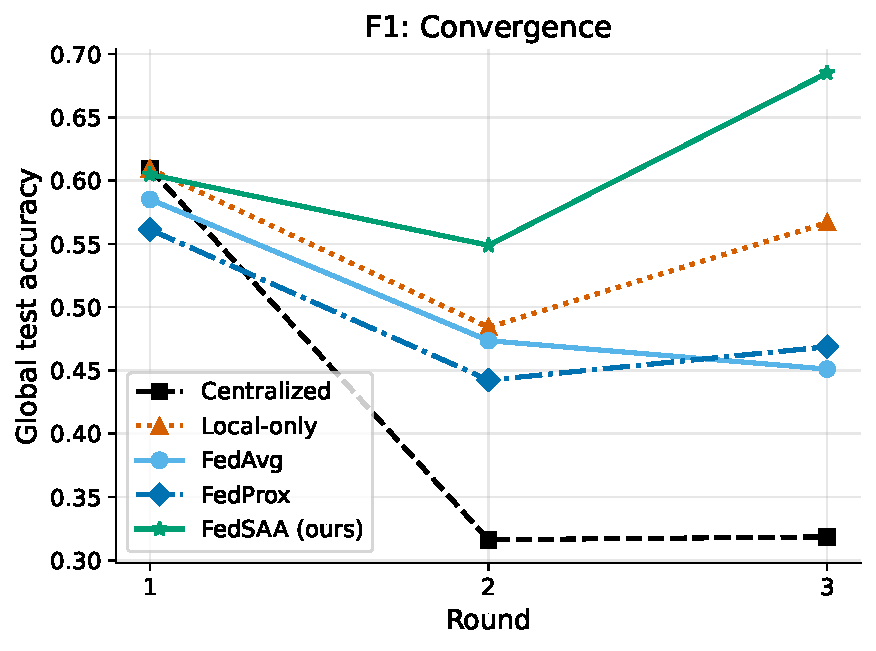
\includegraphics[width=0.75\linewidth]{figures/F1_convergence.pdf}
  \caption{Convergence: global test accuracy vs.\ round.}
  \label{fig:f1}
\end{figure}

\begin{figure}[t]
  \centering
  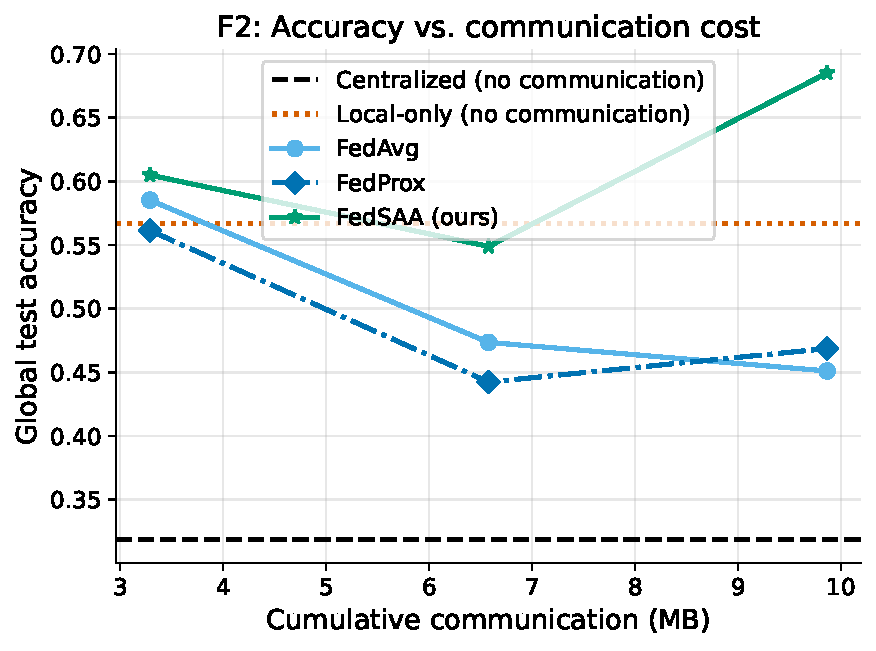
\includegraphics[width=0.75\linewidth]{figures/F2_accuracy_vs_comm.pdf}
  \caption{Accuracy vs.\ cumulative communication (MB).}
  \label{fig:f2}
\end{figure}

\begin{figure}[t]
  \centering
  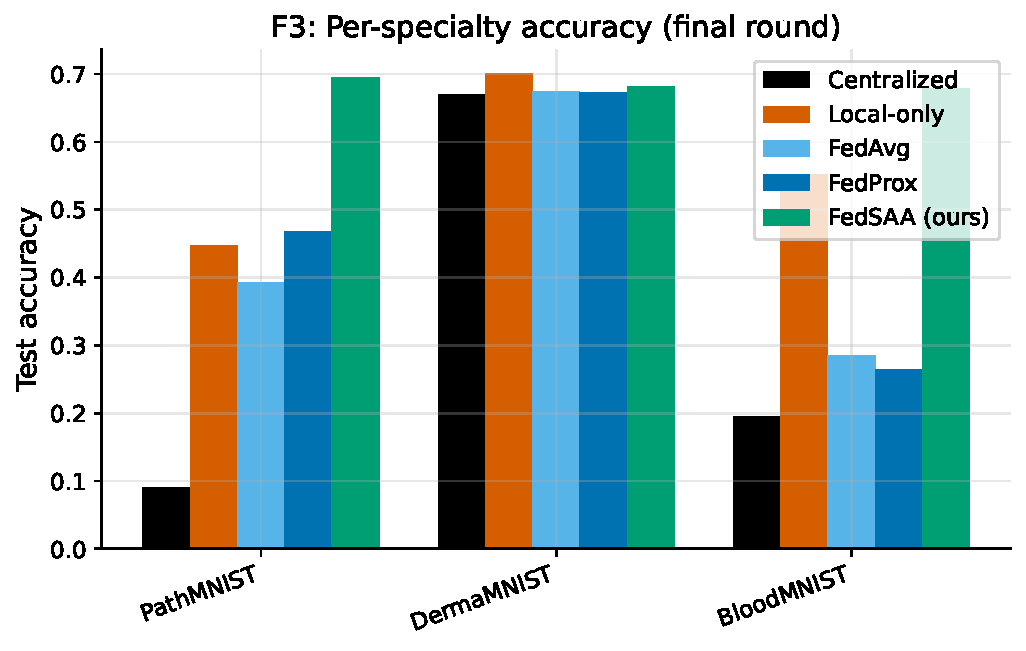
\includegraphics[width=0.9\linewidth]{figures/F3_per_specialty_bars.pdf}
  \caption{Final-round per-specialty accuracy, by method.}
  \label{fig:f3}
\end{figure}

\todo{interpret the Centralized baseline's poor performance -- this reflects an optimization
instability (single shared LoRA adapter, unscheduled lr=0.01 SGD on pooled heterogeneous
batches) flagged during pipeline development, not a fundamental ceiling; revisit with a
tuned/decayed LR before treating Centralized as a true upper bound.}

\subsection{Efficiency}

\begin{table}[t]
\centering
\caption{Efficiency: trainable parameter count (LoRA + one client head), per-round and total communication, and rounds needed to reach 90\% of that method's own best observed accuracy.}
\label{tab:efficiency}
\begin{tabular}{lcccc}
\toprule
Method & Trainable Params & MB/Round & Rounds to 90\\% of own best & Total Comm. (MB) \\
\midrule
Centralized & 148,309 & 0.000 & 1 & 0.00 \\
Local-only & 148,309 & 0.000 & 1 & 0.00 \\
FedAvg & 148,309 & 3.289 & 1 & 9.87 \\
FedProx & 148,309 & 3.289 & 1 & 9.87 \\
FedSAA (ours) & 148,309 & 3.289 & 3 & 9.87 \\
\bottomrule
\end{tabular}
\end{table}


\todo{``rounds to 90\% of own best'' is relative to each method's own final accuracy, not a
shared absolute target -- useful for convergence speed, not cross-method accuracy comparison
(that is Table~\ref{tab:main_results}).}

\subsection{Ablations}

\begin{table}[t]
\centering
\caption{FedSAA ablation over $\lambda$, $\tau$, rank $r$, and client fraction $C$ (mean$\pm$std across seeds).}
\label{tab:ablations}
\begin{tabular}{lcccccc}
\toprule
$\lambda$ & $\tau$ & rank $r$ & $C$ & Global Acc. & Macro-F1 & AUC \\
\midrule
0 & 0.1 & 4 & 1.0 & 0.619$\pm$0.000 & 0.415$\pm$0.000 & 0.834$\pm$0.000 \\
0.5 & 0.1 & 2 & 1.0 & 0.319$\pm$0.000 & 0.126$\pm$0.000 & 0.766$\pm$0.000 \\
0.5 & 0.1 & 4 & 1.0 & 0.605$\pm$0.000 & 0.404$\pm$0.000 & 0.838$\pm$0.000 \\
0.5 & 0.1 & 8 & 1.0 & 0.639$\pm$0.000 & 0.458$\pm$0.000 & 0.881$\pm$0.000 \\
0.5 & 0.1 & 16 & 1.0 & 0.605$\pm$0.000 & 0.437$\pm$0.000 & 0.859$\pm$0.000 \\
1 & 0.1 & 4 & 1.0 & 0.581$\pm$0.000 & 0.364$\pm$0.000 & 0.815$\pm$0.000 \\
\bottomrule
\end{tabular}
\end{table}


\begin{figure}[t]
  \centering
  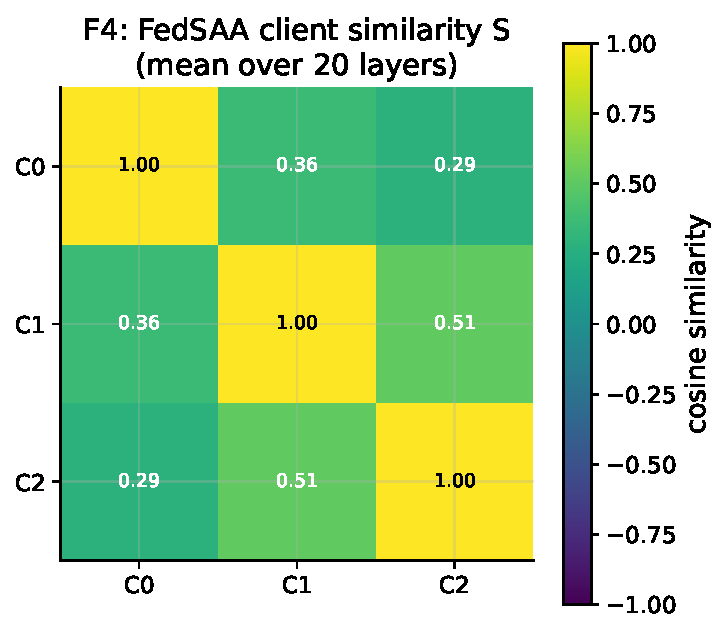
\includegraphics[width=0.7\linewidth]{figures/F4_similarity_heatmap.pdf}
  \caption{FedSAA client similarity matrix $S$ (mean over 20 LoRA layers, final round).}
  \label{fig:f4}
\end{figure}

\begin{figure}[t]
  \centering
  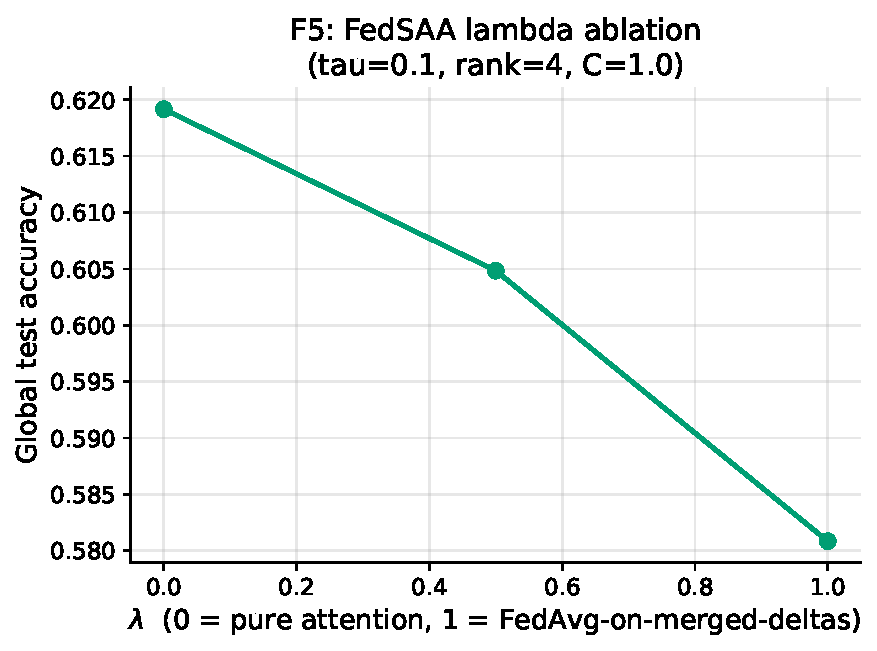
\includegraphics[width=0.7\linewidth]{figures/F5_lambda_ablation.pdf}
  \caption{FedSAA $\lambda$ ablation.}
  \label{fig:f5}
\end{figure}

\begin{figure}[t]
  \centering
  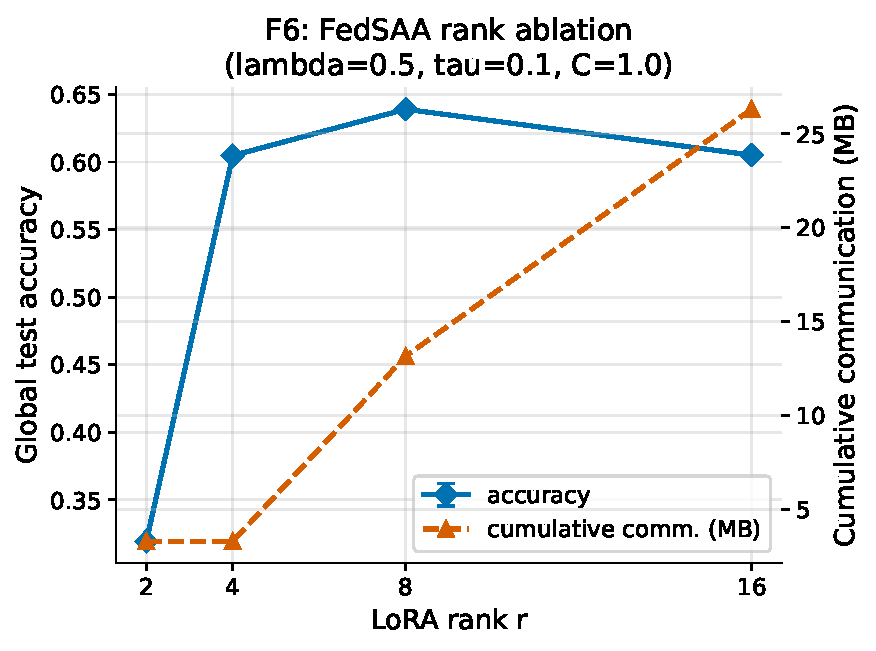
\includegraphics[width=0.7\linewidth]{figures/F6_rank_ablation.pdf}
  \caption{FedSAA rank $r$ ablation (accuracy vs.\ communication trade-off).}
  \label{fig:f6}
\end{figure}

\begin{figure}[t]
  \centering
  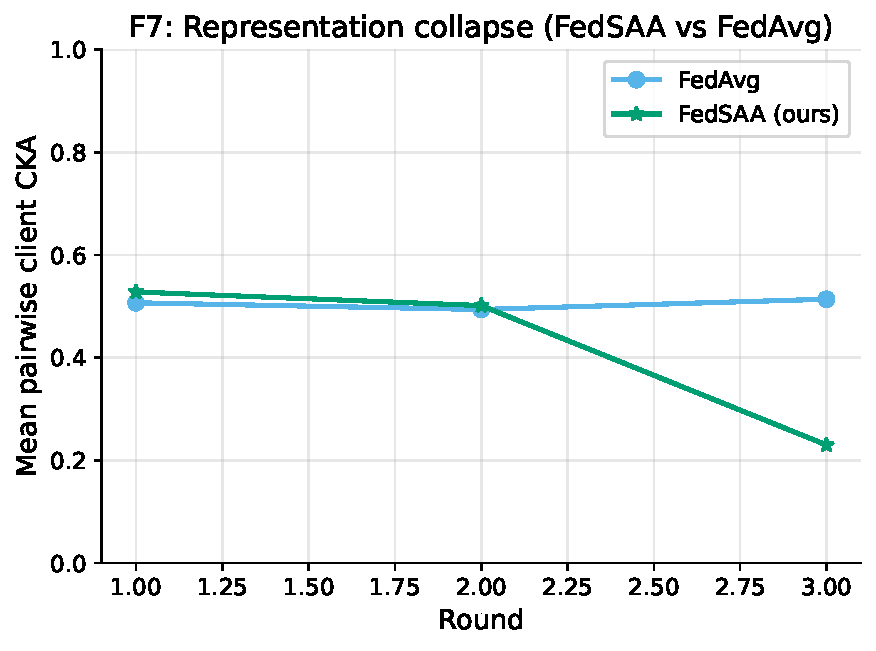
\includegraphics[width=0.7\linewidth]{figures/F7_collapse_cka.pdf}
  \caption{Representation collapse (mean pairwise client CKA vs.\ round), FedSAA vs.\ FedAvg.}
  \label{fig:f7}
\end{figure}

\todo{with only 2-3 points per ablation axis and 1 seed, none of these trends are statistically
meaningful yet -- they demonstrate the ablation \emph{pipeline} works
(\texttt{experiments/runner.py}'s full grid: $\lambda\in\{0,0.25,0.5,0.75,1\}$,
$\tau\in\{0.1,0.5,1\}$, $r\in\{2,4,8,16\}$, $C\in\{0.5,1.0\}$ = 120 configs) but the full grid
$\times$ 3 seeds under \texttt{full\_run.yaml} has not been run. Interpret Figures~\ref{fig:f5}--\ref{fig:f7}
and insert your own reading once it has.}

\section{Limitations}
\label{sec:limitations}

\begin{itemize}
  \item \textbf{All numbers in this draft come from \texttt{configs/local\_debug.yaml}}: 3
    clients (not 5), a 2000-image-per-client subsample cap, and at most 3 rounds with a single
    seed -- deliberately tiny to prove the pipeline end-to-end on an 8\,GB CPU-only laptop.
    \texttt{configs/full\_run.yaml} is the intended real configuration and has not yet been run.
  \item \textbf{Single seed.} Every std-dev in Tables~\ref{tab:main_results}--\ref{tab:ablations}
    is 0.0 because \texttt{seeds=[0]} only -- no variance estimate exists yet.
  \item \textbf{Centralized baseline instability}: macro-F1 collapses to $\sim$0.06 under this
    config's unscheduled SGD lr=0.01 on pooled heterogeneous batches -- a baseline
    hyperparameter/optimization issue, not a property of the data or of FedSAA.
  \item \textbf{Ablation grid coverage}: currently 3 $\lambda$ points and 4 rank points at a
    single $(\tau, C)$ setting each, far short of the full 120-config grid.
  \item \textbf{CPU-only, small backbone}: ResNet-18 at $28\times28$ for laptop feasibility;
    results may not transfer to larger medical backbones/resolutions.
  \item \textbf{MedMNIST as a specialty-heterogeneity proxy}: captures label-space/image-domain
    shift across specialties, not device/scanner variation, within-hospital class imbalance, or
    demographic shift.
\end{itemize}
\todo{add any additional limitations specific to your own reading of the results.}

\section{Conclusion}
\todo{write the actual conclusion once full\_run.yaml results are available. Draft talking
points based on current (smoke-scale) evidence: (1) FedSAA's pipeline runs end-to-end on CPU and
produces personalized, communication-matched LoRA adapters via similarity-attended aggregation;
(2) $\lambda=1$ is verified to exactly reduce to FedAvg-on-merged-deltas, giving a principled
interpolation between personalization and global averaging; (3) early small-scale signal favors
lower $\lambda$ and rank $\approx$8 over the tested range, with meaningfully higher worst-client
accuracy than FedAvg/FedProx at equal communication cost -- but this needs confirmation at
\texttt{full\_run.yaml} scale with multiple seeds before any claim beyond ``the pipeline and
method are implemented correctly.''}

\appendix
\section{Reproducibility}
Code layout, config schema, and CLI: see \texttt{README.md}. To reproduce this draft's numbers:
\texttt{python -m experiments.runner --config configs/local\_debug.yaml --reduced
--rounds-override 3}, then \texttt{python -m src.viz.generate\_figures} and
\texttt{python -m src.viz.generate\_tables} (both \texttt{--config configs/local\_debug.yaml}).
To run the real experiment: \texttt{python -m experiments.runner --config
configs/full\_run.yaml} (see \texttt{experiments/runtime\_estimate.py} for a per-config CPU
runtime warning before committing to a run).

% TODO(author): add a real \bibliography{refs} / \bibliographystyle once citation keys above
% (mcmahan2017fedavg, li2020fedprox, hu2021lora, ...) are backed by an actual .bib file.
\end{document}
